\documentclass{beamer}

\usepackage{wasysym}

\usepackage[utf8]{inputenc}
\usepackage[english]{babel}
\usepackage{url}
\usepackage{listings}
\usepackage{parskip}
\usepackage{cancel}
\usefonttheme{serif}
\setbeamertemplate{navigation symbols}{}
\setbeamertemplate{footline}[page number]{}


\lstset{
  language=Python,
  stepnumber=1,
  breaklines=true,
  basicstyle=\small,
  numbers=left,
  numberstyle=\tiny,
  commentstyle=\color{light-gray},
  escapechar=@,
  mathescape,
}


\begin{document}


\begin{frame}{Outline}
  \begin{enumerate}
  \item Overall architecture
  \item Implementation details
  \item Using the system
  \item Demo
  \end{enumerate}
\end{frame}


\begin{frame}
  \Huge{Overall architecture}
\end{frame}


\begin{frame}{RMI Architecture}
  \begin{center}
    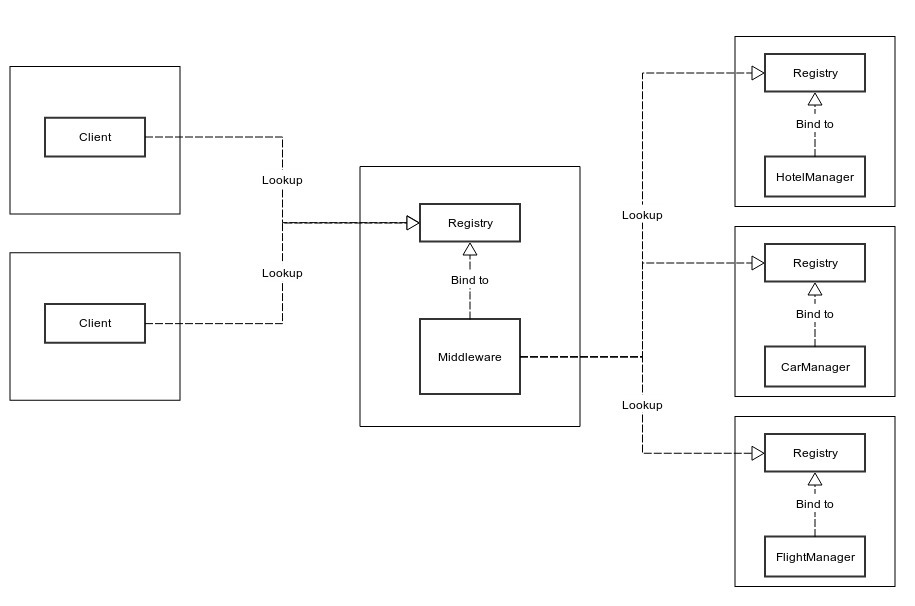
\includegraphics[scale=0.3]{rmi.jpg}
  \end{center}

  (Small difference if a resource manager is in recovery mode)
\end{frame}


\begin{frame}{General architecture}
  \begin{center}
    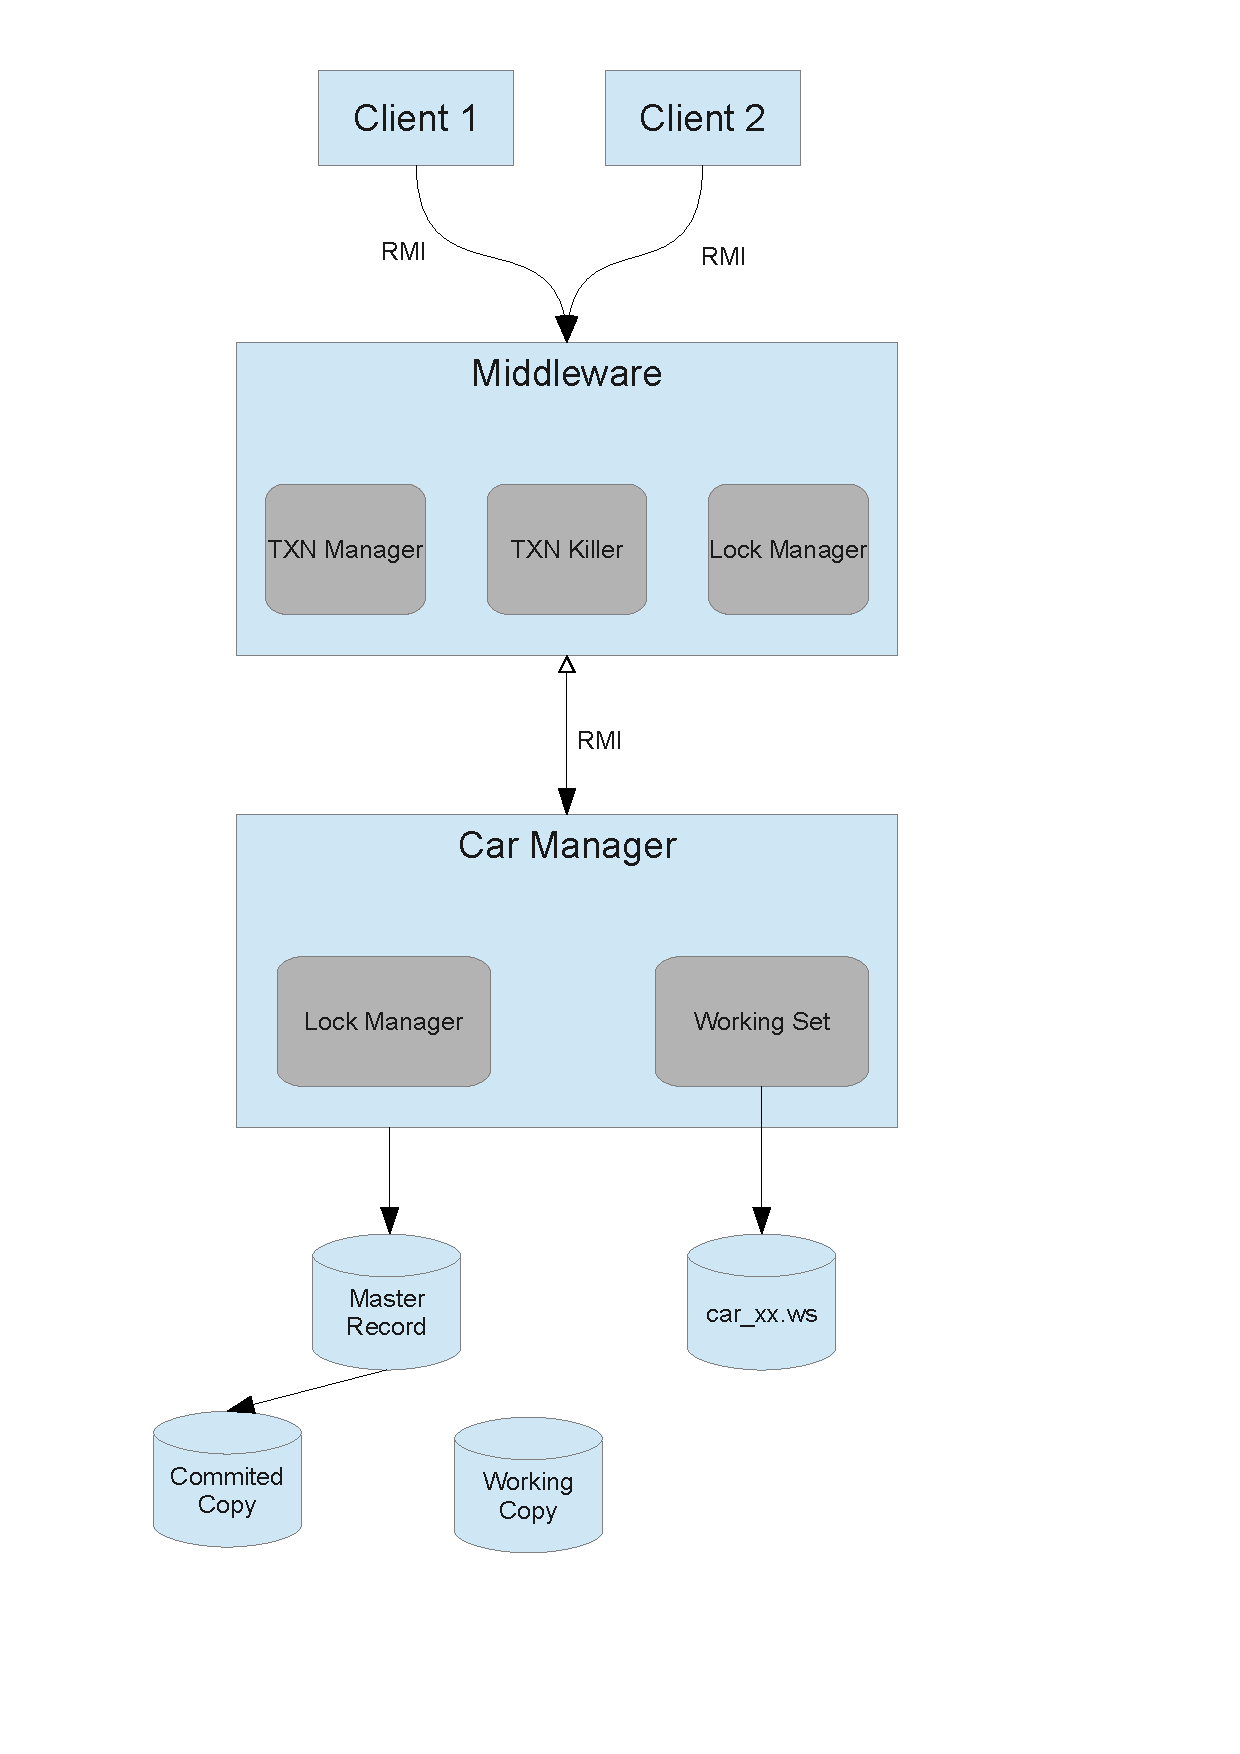
\includegraphics[scale=0.3]{architecture.pdf}
  \end{center}
\end{frame}



\begin{frame}
  \Huge{Implementation details}
\end{frame}


\begin{frame}{Persistence \& Shadowing}

  \emph{/tmp/Group5/} contains master records and databases.


  \begin{itemize}
    \item {\it flightdb.0, flightdb.1}: copies of the flight\footnote{Mutatis mutandis for other resources} data items
    \item {\it flightdb.mr}: points to the commited version
  \end{itemize}

  When a resource manager is started, if the master record and the
  file it points to exist, data is loaded from disk.

  At every commit, data is saved to the file not pointed to by the
  master record and {\tt committed := 1 - committed}
\end{frame}


\begin{frame}{Working Set}
  Three hash tables:

  \begin{itemize}
  \item XID $\to$ Vector$\langle$Command$\rangle$
  \item XID $\to$ Vector$\langle$Item Description$\rangle$
  \item Item Description $\to$ Modified Item
  \end{itemize}


   Writes are stored in the first table and applied to the copy. \\
   Reads are done against the modified item. \\
   To commit: apply commands \\
   To abort: do nothing

   Saved to disk before sending vote.
\end{frame}



\begin{frame}{Transaction Manager}
  Four hash tables:

  \begin{itemize}
  \item XID $\to$ (NOTCOMMITTED $\|$ PHASE1 $\|$ PHASE2)
  \item XID $\to$ Vector$\langle$Involved RM$\rangle$
  \item XID $\to$ TTL
  \item XID $\to$ (COMMIT $\|$ ABORT)
  \end{itemize}

  In charge of 2PC \\
  Logged to disk during 2PC for recovery \\
\end{frame}


\begin{frame}{Two-Phase Commit (Participant view)}

  \begin{center}
    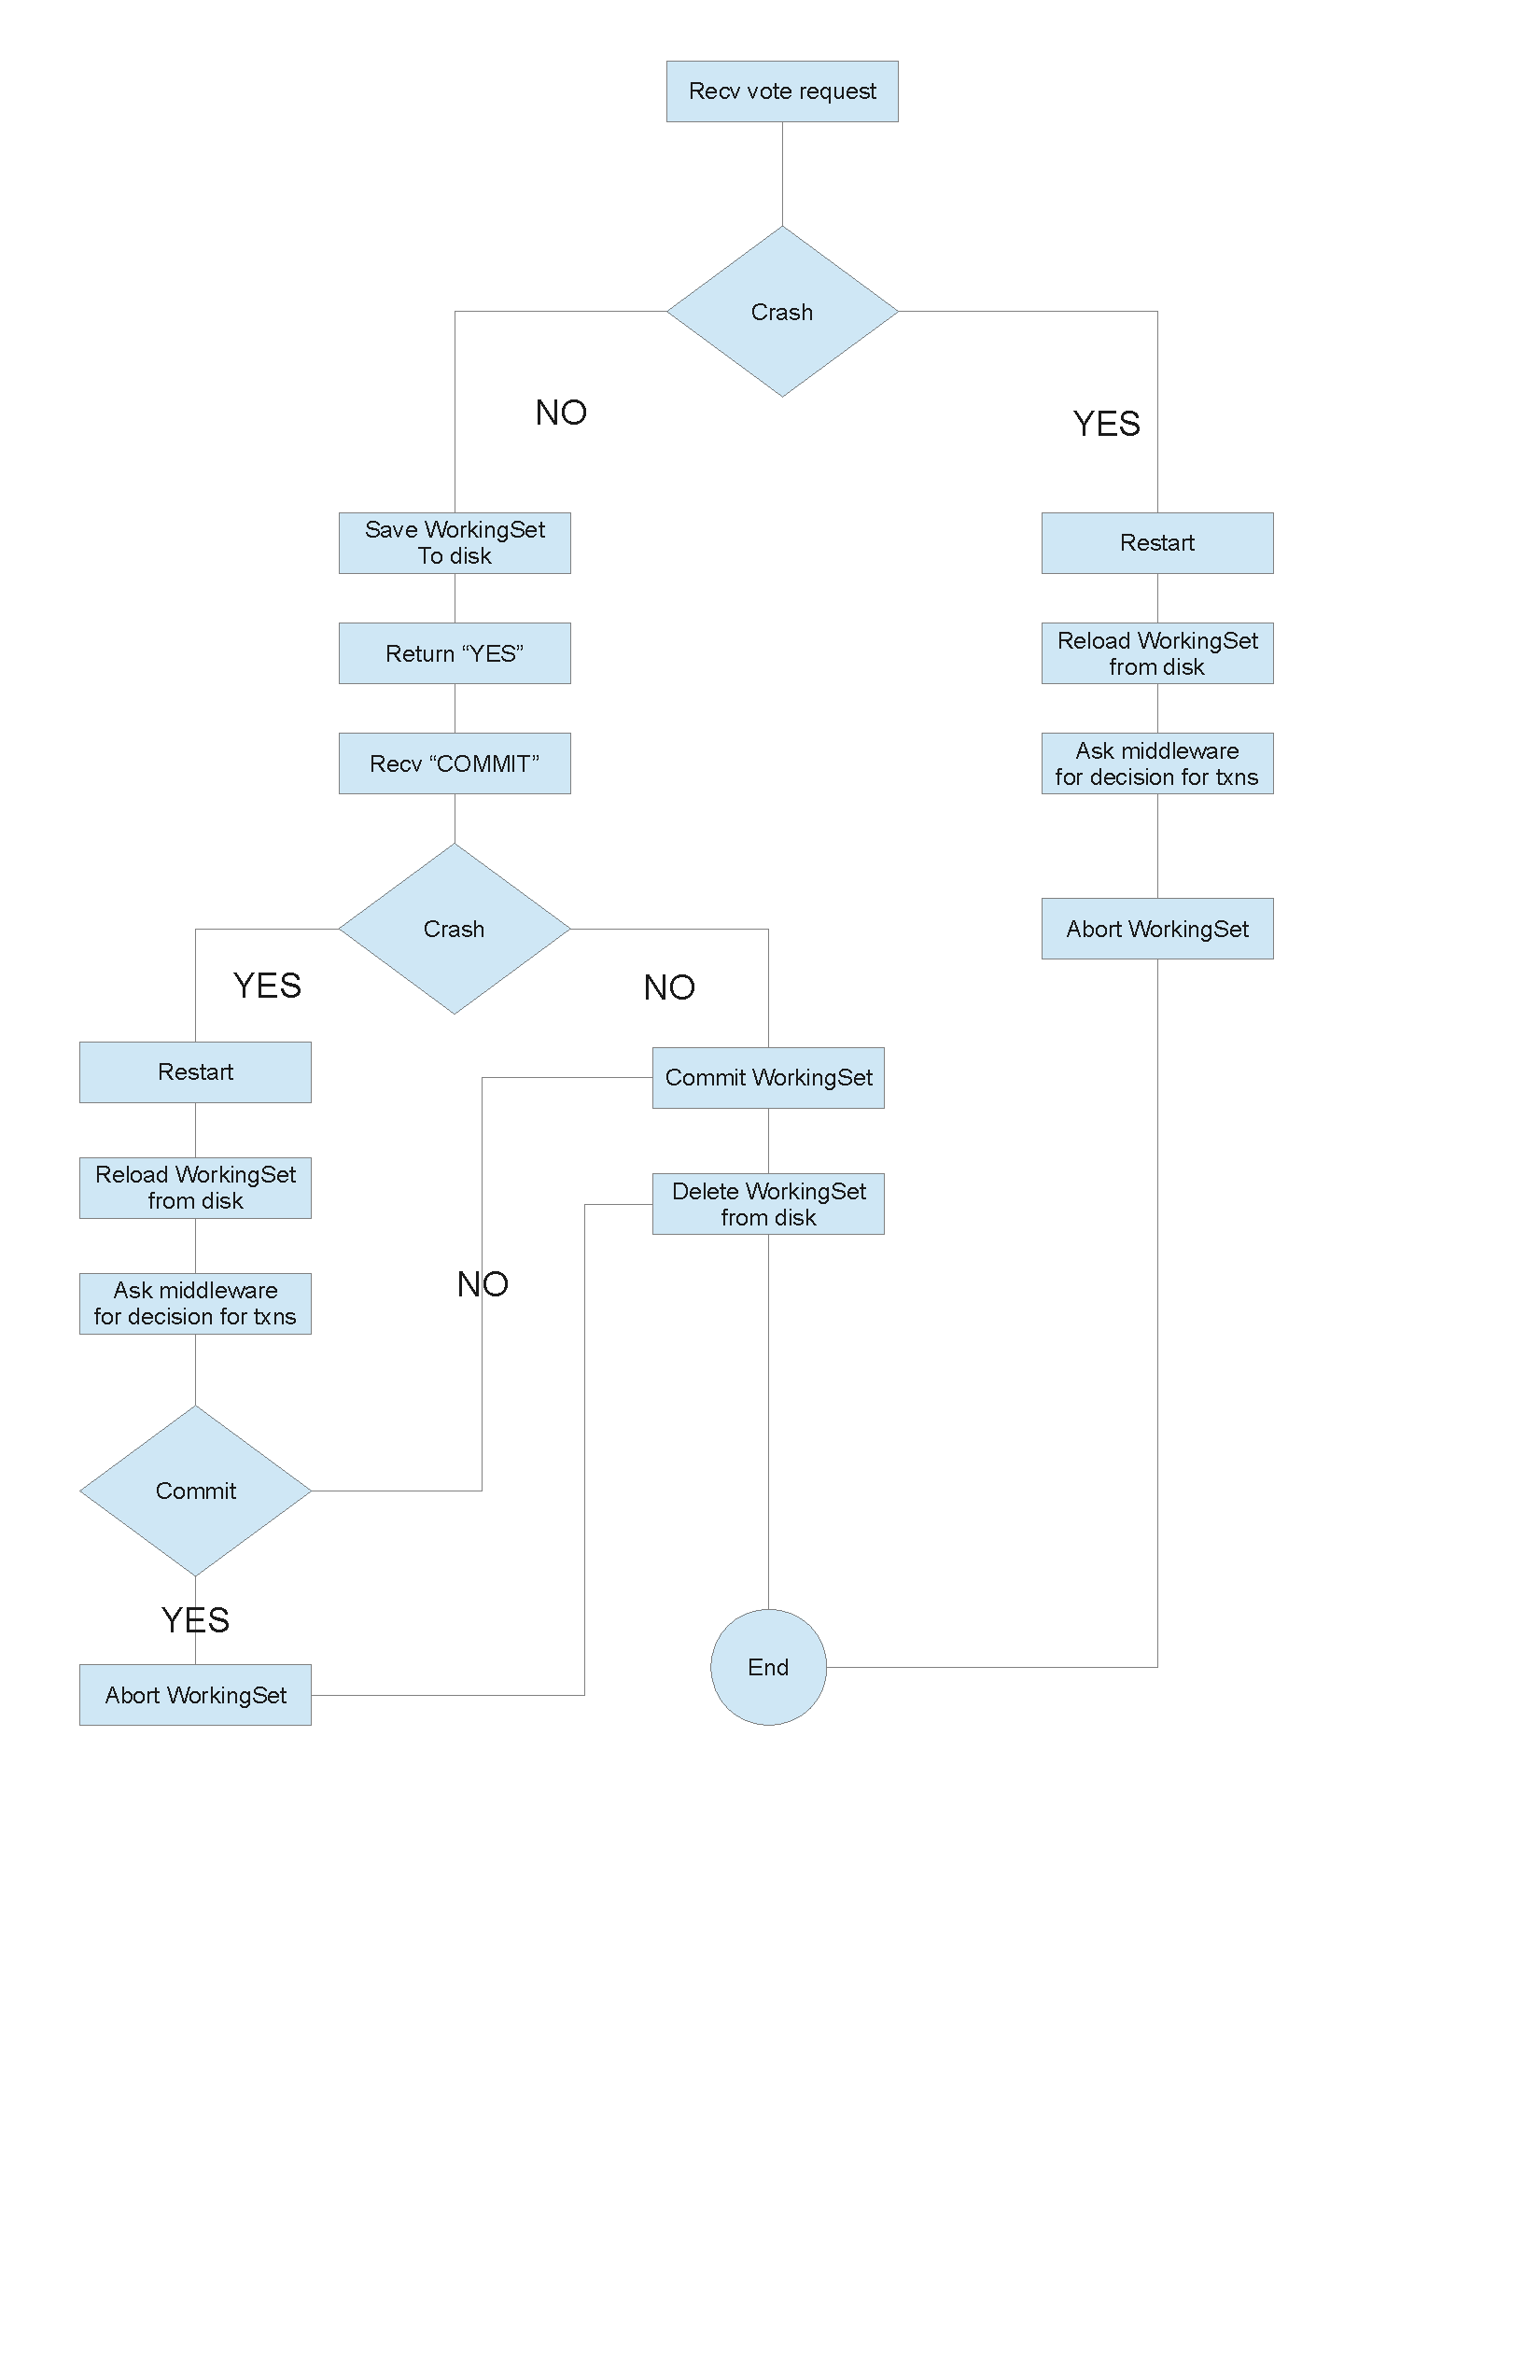
\includegraphics[scale=0.25]{2pc.pdf}
  \end{center}

\end{frame}


\begin{frame}{Two-Phase Commit (Middleware view)}

  \begin{center}
    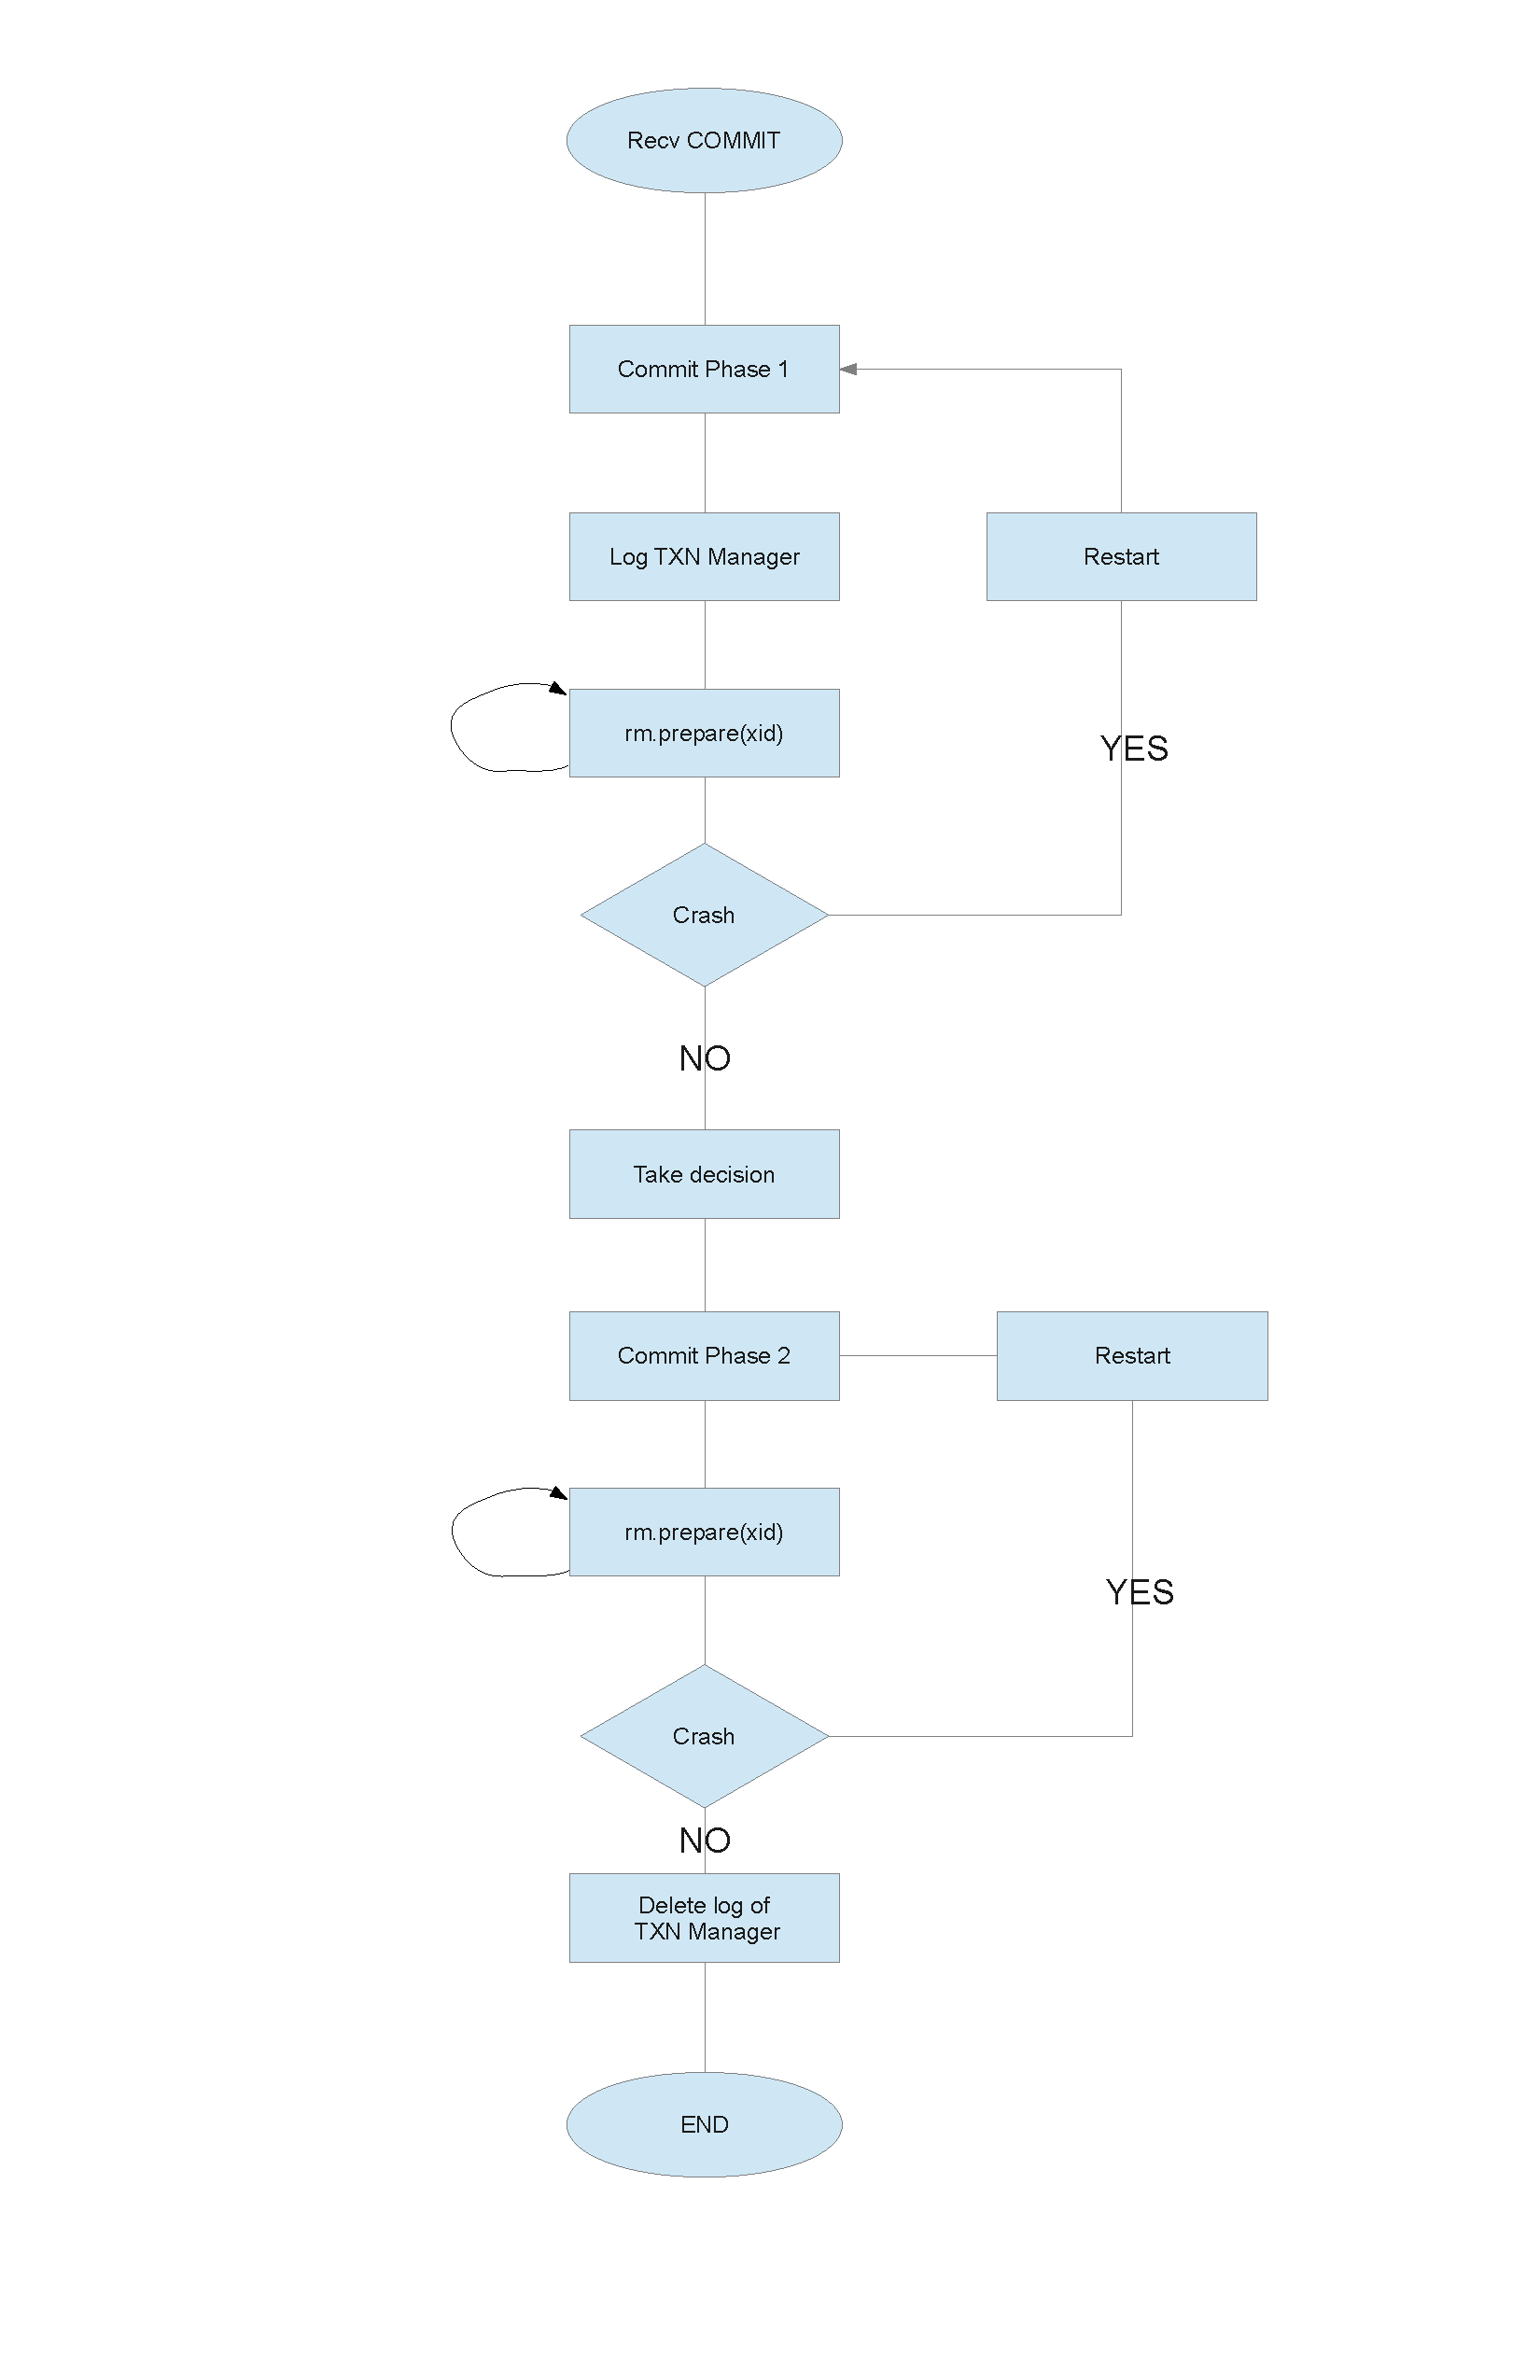
\includegraphics[scale=0.22]{2pc-mw.pdf}
  \end{center}

\end{frame}




\begin{frame}
  \Huge{Using the system}
\end{frame}


\begin{frame}{Makefile system}
  The different components are started with a set of {\it make} rules:

  \small{
    \begin{tabular}{l p{7cm}}
      Make rule & Description \\
      \hline
      {\it make compile} & (Re)compile the whole system \\
      {\it make runcar} \footnote{Idem for flight and hotel managers} & Start a rmiregistry instance and the car manager \\
      {\it make recovercar} & Restart the car manager, providing link to middleware \\
      {\it make runserver} & Start a rmiregistry instance and the middleware \\
      {\it make recoverserver} & Restart the middleware in recovery mode \\
      {\it make runclient } & Start a client and connect to the middleware
    \end{tabular}
  }
\end{frame}


\begin{frame}[t,fragile]
  \frametitle{Crash commands}
  To crash the middleware or a resource manager, extra commands have
  been added to the client.

  {\it crash,$\langle$condition$\rangle$,$\langle$manager$\rangle$}

  Examples:

\begin{verbatim}
# Crash the car manager after
# saving the working set
> crash,P_A_SAVEWS,car

# Crash the transaction manager after
# all vote requests have been sent
> crash,C_A_ALLREPLY,tm
\end{verbatim}
\end{frame}



\begin{frame}
  \Huge{Demo}
\end{frame}


\begin{frame}[fragile,t]
  \frametitle{Demo}
  \framesubtitle{Persistence}

\begin{verbatim}
$ make populate
$ ls /tmp/Group5

> shutdown

# Restart severs

> start
> querycar,xxx,city999
\end{verbatim}
\end{frame}



\begin{frame}[fragile,t]
  \frametitle{Demo}
  \framesubtitle{Shadowing}

\begin{verbatim}
$ ls /tmp/Group5  # Only .mr and .1 files

> start
> itinerary,xxx,11,11,city11,true,true
> commit,xxx

$ ls /tmp/Group5  # Now with .0 files
\end{verbatim}
\end{frame}



\begin{frame}[fragile,t]
  \frametitle{Demo}
  \framesubtitle{Crash car before saving working set}

\begin{verbatim}
> crash,P_B_SAVEWS,car
> start
> itinerary,xxx,22,22,city22,true,true
> commit,xxx   # Boom

$ make recovercar

> start
> querycar,xxx,city22  # 1000 cars
> abort,xxx

\end{verbatim}
\end{frame}


\begin{frame}[fragile,t]
  \frametitle{Demo}
  \framesubtitle{Crash flight after saving working set}

\begin{verbatim}
> crash,P_A_SAVEWS,flight
> start
> itinerary,xxx,33,33,city33,true,true
> commit,xxx   # Boom

$ ls /tmp/Group5/*.ws
$ make recoverflight

> start
> queryflight,xxx,33  # 1000 seats
> abort,xxx
\end{verbatim}
\end{frame}


\begin{frame}[fragile,t]
  \frametitle{Demo}
  \framesubtitle{Crash hotel after sending vote}

\begin{verbatim}
> crash,P_A_COMMITRECV,hotel
> start
> itinerary,xxx,44,44,city44,true,true
> commit,xxx   # Boom

$ make recoverhotel

> start
> queryroom,xxx,city44  # 999 rooms!
> abort,xxx
\end{verbatim}
\end{frame}





\begin{frame}[fragile,t]
  \frametitle{Demo}
  \framesubtitle{Crash middleware during phase 1}

\begin{verbatim}
> crash,C_A_ALLREPLY,tm
> start
> itinerary,xxx,55,55,city55,true,true
> commit,xxx   # Boom

$ make recoverserver

> start
> querycustomer,xxx,55  # Everything's there!
> abort,xxx
\end{verbatim}
\end{frame}



\begin{frame}[fragile,t]
  \frametitle{Demo}
  \framesubtitle{Crash middleware during phase 2}

\begin{verbatim}
> crash,C_A_ALLCOMMIT,tm
> start
> itinerary,xxx,66,66,city66,true,true
> commit,xxx   # Boom

$ make recoverserver

> start
> querycustomer,xxx,66  # Everything's there!
> abort,xxx
\end{verbatim}
\end{frame}




\end{document}
